\documentclass [a4paper,final,conference,10pt]{IDAACS}
\usepackage[utf8]{inputenc}
\usepackage[english]{babel}
\usepackage{amsmath}
\usepackage{graphicx}
\usepackage{multirow}
\usepackage{cite}
\usepackage{pgfplots}
\usepackage{pgfplotstable}
%\title{Effective Parallelization of Mixed-Critical Software to Distributed Heterogeneous Mutlicoresystems}
%\subtitle{
%	Approaching Challenges of Automotive Constrains: Partial Realtime, Safety, Affinity and Connectivity}
%Bare-Metal and OS-based 
%\title{Constrained Parallelization of Mixed-Critical Applications to Distributed Heterogeneous Hardware}
\title{Constrained Mixed-Critical Parallelization for Distributed Heterogeneous Systems}
\author{
%	No authors given for review
\IEEEauthorblockN{Robert Höttger, Mustafa Özcelikörs, Lukas Krawczyk, Philipp Heisig, Carsten Wolff, Burkhard Igel}
%						Third Author's Name\IEEEauthorrefmark{2}}
\IEEEauthorblockA{IDiAL Institute - Dortmund University of Applied Sciences and Arts, \\\{robert.hoettger, mustafa.ozcelikors, lukas.krawczyk,  philipp.heisig, carsten.wolff, igel\}@fh-dortmund.de \\ www.idial.institute 
%						\IEEEauthorrefmark{2}Affiliation, Postal address, e-mail, Web address (URL)\\
%						\IEEEauthorrefmark{3}Affiliation, Postal address, e-mail, Web address (URL)\\
	}
}
\begin{document}
\maketitle

\let\thefootnote\relax\footnotetext{As part of the AMALTHEA4public project, this work has been funded by the German Federal Ministry of Education and Research - BMBF, under funding no. $01|S14029K$}

\begin{abstract}
Distributing software effectively to multi core, many core, and distributed systems has been studied for decades and still advances successively driven by domain specific constraints. Programming vehicle ECUs is one of the most constrained domains that just recently approached the need for concurrency due to advanced driver assistant systems or autonomous driving approaches. In this paper, various challenges for such systems are outlined, discussed, and solutions are given upon instruction precise modeling, affinity constrained distribution, and effective software parallelization. The solutions are compared upon bare-metal and OS based implementations while considering fixed priorities for sequential, OS based, and APP4MC scheduling. The latter case has been published at \cite{ICPDSSE} and evolved to consider affinity constraints, SWC-based partitioning and communication cost related mapping. Results show that using APP4MC based distributions on a distributed heterogeneous system outperforms available approaches for mixed-critical applications.
%TODO percent
\end{abstract}

\begin{IEEEkeywords}
Constrained parallelization, heterogeneous systems, distributed systems, multicore, parallel embedded systems
\end{IEEEkeywords}

\section{Introduction}
Especially the automotive domain requires lots of constraints originating from different safety, security, timing, or similar requirements. The verification, validation, testing, and simulation stack requires dozens of tools and the consideration of established architectures, standards, models, and assessments to address product line supporting, consistent, modular, and scalable software. However, these efforts lack in transparency likewise the comprehensive understanding of applications. Recent approaches such as APP4MC\cite{app4mc}
%\footnote{\underline{A}pplication \underline{P}latform \underline{P}roject for Multi and Manycore, http://eclip.se/a7, access February 2017} 
already address this challenge and try to provide a common adaptable platform based on AUTOSAR\cite{autosar} while providing a standardized data model. Any specific commercial or proprietary tooling is supposed to be integrable in order to provide seamless interaction with provided tooling such as product line management, requirements engineering, partitioning, mapping, testing, and more. 

In this paper, we use the open source APP4MC environment in order to address both industrial and research related models while evaluating our new developments not only regarding model results but also to validate result among a specific use case described in section \ref{sec:rccar}. The RC-Car is an advanced demonstrator that features 16 100MHz logical cores (XMOS ExplorerKit, XCore-200) 
%2 instructions per cycle see (more details): https://www.xmos.com/download/private/xCORE-Architecture-Flyer%281.1%29.pdf
%2000MIPS 16 core: https://www.xmos.com/download/private/xCORE-200-XE-Product-Brief%281.2%29.pdf
%--> 125MIPS per logical core, --> 1,25 instructions per cycle?
combined with four cores clocked at 1200MHz (Raspberry Pi 3, ARM CoreTex-A53). With using APP4MC, we show that automatic OS driven distributions not always create the most efficient results.

The further remainder of this paper is structured as follows: Section \ref{sec:app4mc} roughly describes the environment this contribution is based upon and its specifics among constraints and instructions. Afterwards, Section \ref{sec:rccar} illustrates capabilities and properties of the RC-Car demonstrator as well as its distributed architecture and concurrency capabilities. Subsequently, Section \ref{sec:eval} evaluates the results and benefits gained from using APP4MC for an automatic, constrained based parallelization of a mixed critical application, while Section \ref{sec:relatedWork} reviews related work.  %outlines the specific developments and solutions to precise modeling and software parallelization that is evaluated and compared to related approaches in section \ref{sec:eval}. 
Finally, Section \ref{sec:concl} concludes this paper's contributions and discusses benefits, disadvantages, possible extensions, and promising outlooks that potentially advance the current approach.

\section{APP4MC}
\label{sec:app4mc}
%FOCUS Constraints
APP4MC is an open source project for developing multi and many core systems primarily for the automotive domain. Instead of describing its different purposes and features, the focus of this section is on the required steps to utilize APP4MC parallelization capabilities \cite{ICPDSSE}, i.e. partitioning and mapping. Those processes have been advanced in recent years to consider affinity, allocation, and safety constraints among others. Dealing with safety constraints ensures that tasks with a specific \underline{A}utomotive \underline{S}afety \underline{I}ntegrity \underline{L}evel (ASIL) are allocated to processing units (cores) featuring the corresponding ASIL level. Allocation constraints are considered the same way, except that instead of ASIL levels properties such as \underline{F}loating \underline{P}oint \underline{U}nit (FPU) connectivity, cache memory size, processing frequency or others are investigated. Affinity constraints are evaluated within the partitioning process since runnables, i.e. smallest executable units, have to be kept in the same partition that are later on resolved to tasks. This paper's application, i.e. the RC-Car, features all of those constraints. Affinity has to be kept for instance regarding the light system state task and the \underline{P}ulse \underline{W}idth \underline{M}odulation (PWM) signal generation (timer) tasks since their distribution would cause implementation and communication overheads. Since there are tasks that continuously check the core utilization on each X-Core Tile, those tasks feature an allocation constraint to each X-Core Tile. Finally, due to the fact that the RC-Car performs image processing from a camera as well as real time tasks for motor control, steering, and bluetooth based communications, we define all tasks that are crucial for safe driving as being safety critical (safety constraint) and bind them to the real time capable XMOS board. 

Apart from the constraints, software and hardware descriptions are required. While the hardware model is created manually, a C/CPP parser was used to receive necessary AMALTHEA software model data, i.e. runnables, labels, label accesses, activations, runnable calls, \underline{I}nterrupts \underline{S}ervice \underline{R}outines (ISRs), Semaphores, and more for the Raspberry Pi (RPI) implementations. Excerpts of those models are shown in Figure~\ref{fig:model}. While the RPI already features 247 Runnables and more, XMOS implementations were modeled on a higher level upon threads only, that correspond tasks. Those count 30 in total where profiling was performed via counting assembler instructions and using individual scripts for profiling.

\begin{figure}[bth]
	\centering
	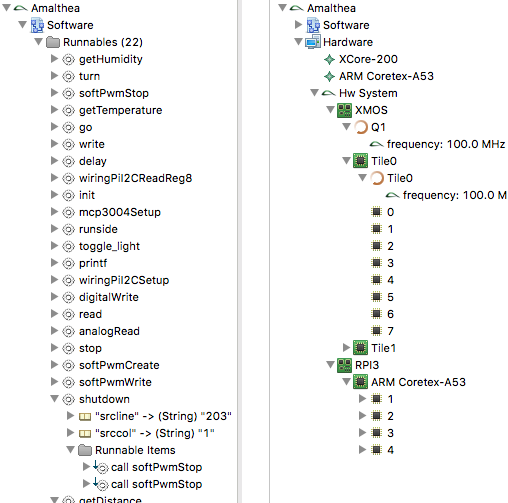
\includegraphics[scale=0.34]{images/models.png}
	\caption{\label{fig:model}AMALTHEA software and hardware models (excerpts) for the RC-Car}
\end{figure}

%TODO insert how instructions of XMOS threads were found out
%The created scripts or applications need to be modeled precisely with APP4MC in order to get more accurate results. 
More precisely, the Linux OS provides a set of important kernel-level tools as well as methods to analyze processes, threads, and binaries. Consequently, we use those to model the implementations and transform them to Amalthea models. Since the amount of functions i.e. smallest executable units that are transformed to runnables, often reaches beyond 100, the transformation is required to be done automatically by a parser or script. The tool '\textbf{objectdump}' meets this tasks due to its capability to derive disassembled runnables from binary files created from C or C++ files. While this stays quite straight forward, deriving instructions, deadlines, or WCET has to be addressed by specific profiling tools that handle binary object disassembly. For this purpose the '\textbf{perf}' tool fits our need most and has been integrated to script to derive the required instructions. Furthermore, via accessing the kernel folder '\textbf{proc}' we derive affinity constraints to keep some specific functions from being separated during partitioning or mapping processes. 
%The first required step that is needed in order to properly model the runnables and tasks is getting the proper number of instructions by either looking at disassembly of binary objects or using profiling tools. 
%In order to profile the dynamic processes, which are one of the greatest parts in our application, the tool 'perf' has been used. 
%A linux system bash script has been created in order to get the dynamical instructions by making use of this tool.
%One could also make use of the kernel folders in Linux such as 'proc' in order to define constraints for the processes while modeling them in APP4MC.
%Furthermore, the runnables within C/C++ applications are disassembled and analyzed by using the tool 'objdump', which creates disassembled runnables from binary files.
Linux provides other tools such as '\textbf{top}' and '\textbf{taskset}', which are also crucial to the development of multi-core systems. The tool '\textbf{top}' is used for the process monitoring, whereas the tool '\textbf{taskset}' is used for thread to core mapping in order to manage the multi-core distribution provided by APP4MC.
%In the RC-CAR, the aforementioned tools are used in order to manage a multi-process system distributed on multiple cores.
The specific mapping on the RC-CAR is finally considered automatically by a created Python script, which utilizes a generated C file from APP4MC and accordingly distributes the tasks using Linux's '\textbf{taskset}'.

Before the partitioning and mapping processes can be configured and executed, one of the most challenging key property has to be added to runnables, i.e. the above mentioned affinity, allocation, and safety constraints.
%TODO  constraints modeling
\section{RC-Car}
\label{sec:rccar}
The current Raspberry Pi distribution includes processes for the touchscreen, ethernet communication, core utilization reader, mjpg streamer, vnc application, apache2, OpenCV\cite{opencv} image processing, and additional cyclewaster. The latter processes can be added in order to push the core utilization to a maximum and consider high workload. The effective distribution by APP4MC is crucial to provide deadline violation free program execution. 

The XMOS tasks focus on necessary real time implementations. Scheduling on the XMOS is non preemptive and allows a better determinism as well as easier \underline{W}orst \underline{C}ase \underline{E}xecution \underline{T}ime (WCET) reasoning due to less context switching and less scheduling jitter \cite{xmos}. However, since our number of tasks exceed the total number of available cores on the XMOS, we had to define high priority tasks, that run on dedicated cores, and low priority tasks that run concurrently with other low level tasks in cooperative multitask manner on common cores (via \textit{combinable} functions in XMOS terminology). The amount of high priority tasks thereby defines the number of cores available for the low priority tasks. 

Figure \ref{fig:arch} shows the basic RC-Car architecture that uses different communication APIs such as Ethernet, I2C, or UART as well as various actuators and sensors to interact with its environment. Its current application is to approach autonomous driving scenarios.
\begin{figure}[bth]
	\centering
	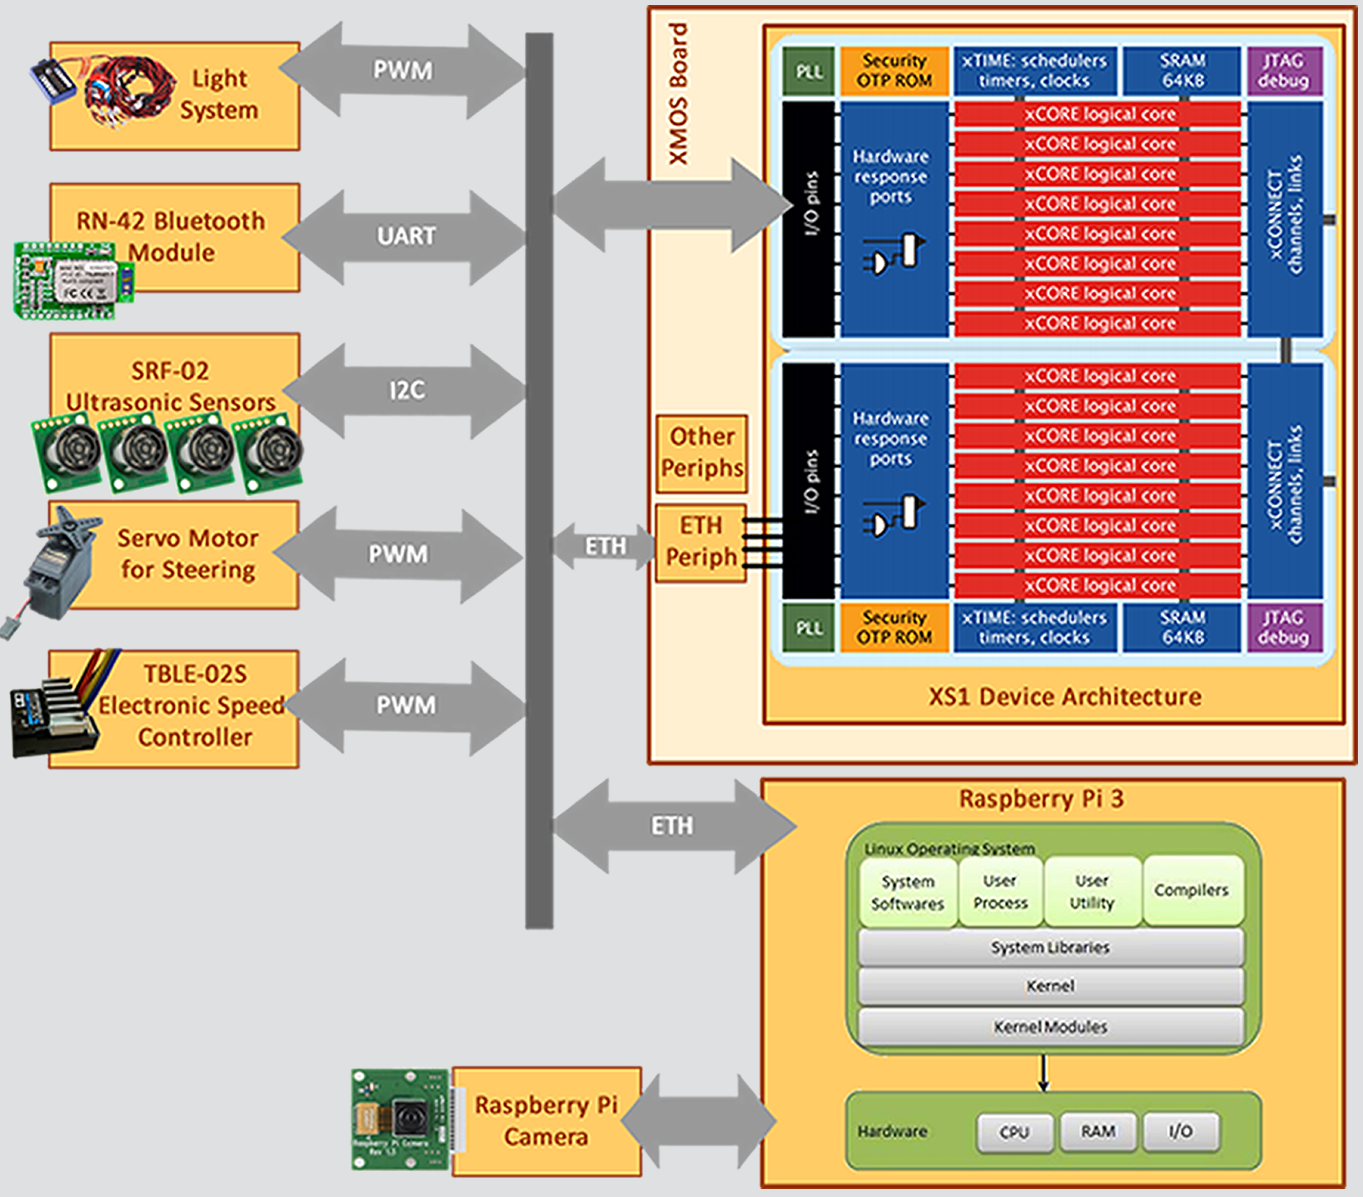
\includegraphics[scale=0.118]{images/hwarch.png}
	\caption{\label{fig:arch}RC-Car architecture, interfaces, sensors, and actuators}
\end{figure}

%EQUATION-----------------------------------------------
%\begin{equation}
%\label{Eq_1}
%\lambda_i = \lim \frac{1}{p} \sum_{t=1}^p \ln \frac{|w_i (t)|}{|w_i (t-1)|}
%\end{equation}

%TODO maybe skip the following chapter
%\section{Precise modeling and Software Parallelization}
%\label{sec:impl}

%FIGURE-----------------------------------------------
%\begin{figure}[bth]
%\centering
%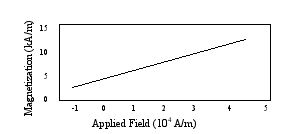
\includegraphics[scale=0.6]{images/Fig1.png}
%\caption{\label{Fig_Magnet}Magnetization as a function of applied field. Note 
%how the caption is centered in the column.}
%\end{figure}

%TABLE-----------------------------------------------
%\begin{table}[htb]
%\caption{Table Type Styles}
%\label{Table_I}1
%\centering
%\begin{tabular}{|p{1.2cm}|p{1.5cm}|p{1.5cm}|p{1.5cm}|}
%\hline
%\multirow{2}{1.2cm}{\textbf{Type Size (pts.)}} & \multicolumn{3}{|c|}{\textbf{Appearance}}\\
%\cline{2-4}
% & \textbf{\textit{Regular}}&\textbf{\textit{Bold}}&\textbf{\textit{Italic}}\\
%\hline
%8 & References, table header, footnotes, text subscripts, and superscripts &&\\
%\hline
%\end{tabular}
%\end{table}

\section{Evaluation}
\label{sec:eval}
The following chart (Figure \ref{fig:dischart}) shows results of three different software distribution scenarios on the RC-Car obtained from separate utilization tracker threads. \\
For clarity purposes, the XMOS logical cores were combined to the corresponding tiles since their separation would result in less clarity as well as lessen the physical accordance. Hence, each color on a XMOS tile can consume up to 12,5\% maximal tile utilization, such that a tile is only fully utilized if all 8 cores fully express 12,5\% core utilization.
\begin{figure*}[t!]\centering
	\newcounter{groupcount}
	\pgfplotsset{
		legend style={at={(axis cs:24,0)},anchor=south west},
		draw group line/.style n args={5}{
			after end axis/.append code={
				\setcounter{groupcount}{0}
				\pgfplotstableforeachcolumnelement{#1}\of\datatable\as\cell{%
					\def\temp{#2}
					\ifx\temp\cell
					\ifnum\thegroupcount=0
					\stepcounter{groupcount}
					\pgfplotstablegetelem{\pgfplotstablerow}{X}\of\datatable
					\coordinate [yshift=#4] (startgroup) at (axis cs:\pgfplotsretval,0);
					\else
					\pgfplotstablegetelem{\pgfplotstablerow}{X}\of\datatable
					\coordinate [yshift=#4] (endgroup) at (axis cs:\pgfplotsretval,0);
					\fi
					\else
					\ifnum\thegroupcount=1
					\setcounter{groupcount}{0}
					\draw [
					shorten >=-#5,
					shorten <=-#5
					] (startgroup) -- node [anchor=base, yshift=0.5ex] {#3} (endgroup);
					\fi
					\fi
				}
				\ifnum\thegroupcount=1
				\setcounter{groupcount}{0}
				\draw [
				shorten >=-#5,
				shorten <=-#5
				] (startgroup) -- node [anchor=base, yshift=0.5ex] {#3} (endgroup);
				\fi
			}
		}
	}
	\begin{tikzpicture}
	\pgfplotstableread{
		X Gp D1 Name RPI C0 C1 C2 C3 C4 C5 C6 C7
		1 Sequential RPI Core0 100 0 0 0 0 0 0 0 0 
		2   Sequential RPI Core1 0 0 0 0 0 0 0 0 0
		3   Sequential RPI Core2 0 0 0 0 0 0 0 0 0
		4   Sequential RPI Core3 0 0 0 0 0 0 0 0 0
		6   Sequential XMOS Tile0 0 12.5 0 0 0 0 0 0 0 
		7   Sequential XMOS Tile1 0 0 0 0 0 0 0 0 0 
		9 Automatic RPI Core0 96 0 0 0 0 0 0 0 0
		10  Automatic RPI Core1 49.6 0 0 0 0 0 0 0 0
		11  Automatic RPI Core2 22.9 0 0 0 0 0 0 0 0
		12  Automatic RPI Core3 15.1 0 0 0 0 0 0 0 0
		14  Automatic XMOS Tile0 0 12.5 12.5 12.5 12.5 12.5 10 9 12.5 
		15  Automatic XMOS Tile1 0 12.5 12.5 12.5 12.5 12.5 12.5 12.5 10 
		17  APP4MC RPI Core0 47 0 0 0 0 0 0 0 0
		18  APP4MC RPI Core1 34 0 0 0 0 0 0 0 0
		19  APP4MC RPI Core2 44 0 0 0 0 0 0 0 0
		20  APP4MC RPI Core3 60 0 0 0 0 0 0 0 0
		22  APP4MC XMOS Tile0 0 12.5 12.5 5 5 8 6 14 7 
		23  APP4MC XMOS Tile1 0 8 9 10 11 9 8 12 10 
	}\datatable
	\begin{axis}[
	axis lines*=left, ymajorgrids,
	width=15cm, height=6cm,
	ymin=0,
	ybar stacked,
	bar width=7pt,
	xtick=data,
	xticklabels from table={\datatable}{Name},
	xticklabel style={rotate=90,xshift=-7ex,anchor=mid east},
	draw group line={D1}{RPI}{RPI\,}{-7ex}{5pt},
	draw group line={D1}{XMOS}{XMOS\,}{-7ex}{5pt},
	draw group line={Gp}{Sequential}{Sequential}{-4ex}{7pt},
	draw group line={Gp}{Automatic}{Automatic}{-4ex}{7pt},
	draw group line={Gp}{APP4MC}{APP4MC}{-4ex}{7pt},
	after end axis/.append code={
		\path [anchor=base east, yshift=0.ex]
		(rel axis cs:0,0) node [yshift=-7ex] {Board}
		(rel axis cs:0,0) node [yshift=-4ex] {Distribution};
	}
	]
	
	\addplot table [x=X, y=RPI] {\datatable}; \addlegendentry{RPI}
	\addplot table [x=X, y=C0] {\datatable}; \addlegendentry{C0}
	\addplot [teal!80!black,fill=teal!50!white] table [x=X, y=C1]{\datatable}; \addlegendentry{C1}
	\addplot [violet!80!black,fill=violet!50!white] table [x=X, y=C2]{\datatable}; \addlegendentry{C2}
	\addplot [pink!80!black,fill=pink!50!white] table [x=X, y=C3]{\datatable}; \addlegendentry{C3}
	\addplot [brown!80!black,fill=brown!50!white] table [x=X, y=C4]{\datatable}; \addlegendentry{C4}
	\addplot [cyan!80!black,fill=cyan!50!white] table [x=X, y=C5]{\datatable}; \addlegendentry{C5}
	\addplot [lightgray!80!black,fill=lightgray!50!white] table [x=X, y=C6]{\datatable}; \addlegendentry{C6}
	\addplot [orange!80!black,fill=orange!50!white] table [x=X, y=C7]{\datatable}; \addlegendentry{C7}
	\end{axis}
	\end{tikzpicture}
	\vspace{-10pt}
	\caption{Core utilization in \% (y-axis) for sequentail, automatic, and APP4MC distribution}
	\label{fig:dischart}
\end{figure*}
The distributed sequential parallelization (left part of Figure \ref{fig:dischart}) shows that each board (RPI \& XMOS) has one fully utilized processing unit. Consequently, applications and tasks can hardly meet their deadlines and execute with very low throughput. In contrast to that, when using the Linux \underline{C}ompletely \underline{F}air \underline{Q}ueuing (CFQ) scheduler without explicitly defining priority or scheduling classes %more info required?
on the RPI as well as the round robin scheduler on the XMOS via \texttt{par} statements, one can experience great benefits due to concurrent progressing on both hardware units (see mid part of Figure \ref{fig:dischart}). Nevertheless, for this case programmers still need to manually separate the real time applications from the non-critical programs and map them to the corresponding processing elements (critical programs to the XMOS, non-critical to the RPI). It is important to note here, that the non-critical tasks still have deadlines to meet in order to assess effectiveness, i.e. that results are produced within a limited time period predefined by requirements.

However, as pointed out earlier in this paper, the automatic distributions are not always the prior choice when targeting efficiency. Deadlines may be met comprehensively (the effect is the same), but long slack times waste processing cycles that could be spent otherwise. The APP4MC distribution (right part of Figure \ref{fig:dischart}) do not only considers any types of constraints but also can be configured to balance load as much as possible such that for instance the total frequency (here on the RPI) could be scaled down to safe energy. Assuming a global \underline{D}ynamic \underline{V}oltage and \underline{F}requency \underline{S}caling (DVFS) feature on the RPI, we measured up to 9\% less energy consumption when commonly reducing the CPU frequencies from 1200MHz to 800MHz while still meeting all deadlines.  %TODO real measurements required; also assumption: DFVS global, since Linus does not allow CPUinfo_min_freq per-core

%in parallel and distributed systems like
\section{Related Work}
\label{sec:relatedWork}
With the advent of multi- or many-core hardware in embedded systems, a lot of work dealing with the efficient distribution of software to the respective cores with regard to specific constraints has been published. Socci et al. \cite{Socci2015} provide an algorithm for multi-processor scheduling of mixed criticality task graphs in synchronous systems through precedence constraints. 
Xiao et al. \cite{Xiao2016} focus on minimizing the energy consumption by scheduling parallel application towards heterogeneous distributed environments based on energy consumption constraints, while Liang et al. \cite{LiXi13} propose an algorithm for reducing the energy consumption of high performance clusters via precedence
constrained without increasing the schedule length. In contrast to the prementioned work, our approach takes several kinds of design constraints, e.g. affinity, allocation or ASIL constraints, into account.

 \cite{Kritikakou2014} 

\section{Conclusion}
\label{sec:concl}
Within this paper, we successfully validated that using APP4MC for efficient mixed-critical software parallelization to distributed heterogeneous systems eases development processes on various levels. Error prone and time consuming manual software distribution can be avoided and utilizing APP4MC results even outperforms OS or compiler based automatic approaches. While the constraint modeling requires certain efforts, it considers crucial requirements emerging from timing, safety, or security demands that are inevitable in modern industrial developments. Our experiments among an 


%TODO maybe more Amalthea paper?
\section*{Acknowledgment}
The authors would like to express their appreciation to the AMALTHEA4public consortium for sharing experience, knowledge, and know-how. Special thanks to 
%\enlargethispage{-7in}
\bibliographystyle{IEEEtran}
\bibliography{ref}
\end{document}